%%%%%%%%%%%%%%%%%%%%%%%%%%%%%%%%%%%%%%%%%%%%%%%%%%%%%%%%%%%%%%%%%%%%%%%%%%
%
% Copyright (c) 2012 Jorge Nunes, All Rights Reserved.
%
%%%%%%%%%%%%%%%%%%%%%%%%%%%%%%%%%%%%%%%%%%%%%%%%%%%%%%%%%%%%%%%%%%%%%%%%%%

\documentclass[11pt]{article}

\usepackage[portuges]{babel}
\usepackage[utf8]{inputenc} 
\usepackage{a4}
\usepackage{amsfonts}
\usepackage{float}
\usepackage{graphicx}





\begin{document}

\section*{Ilha de Koch}

Neste artigo iremos falar muito superficialmente sobre as figuras
geométricas conhecidas como linha de Koch e ilha de Koch. O nome vem
do matemático sueco Helge von Koch, que em 1904 referiu num artigo
pela primeira vez a curva que é hoje conhecida como linha de Koch.





\section{Linha de Koch}

A linha de Koch é uma figura geométrica que nos será útil para definir
a ilha de Koch. Consideremos a sequência de figuras que descrevemos em
seguida. Começamos com um segmento horizontal, com uma unidade de
comprimento.

\begin{figure}[H]
  \centering
  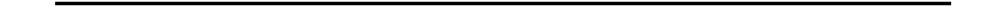
\includegraphics[width=0.3\textwidth]{../images/koch-line-00.pdf}
  \caption{Ponto de partida para a construção da linha de Koch.}
\end{figure}


Em seguida, dividimos este segmento em três partes iguais e
substituimos a parte do meio por outros dois segmentos correspondendo
a dois lados de um triângulo equilátero. Este passo está ilustrado na
figura em baixo. O comprimento de cada um destes 4 segmentos é 1/3
pelo que o comprimento da linha completa é de 4/3.

\begin{figure}[H]
  \centering
  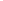
\includegraphics[width=0.3\textwidth]{../images/koch-line-01.pdf}
  \caption{Primeira iteração da construção da linha de Koch.}
\end{figure}


No terceiro passo fazemos algo semelhante ao realizado no segundo
passo, agora para cada um dos 4 segmentos da figura. Cada segmento é
dividido em três e a parte do meio substituida por outros dois
segmentos formando dois lados de um triângulo equilátero. Se no
segundo passo a figura era composta por segmentos de comprimento 1/3
agora os segmentos são de comprimento 1/9 e o comprimento total passou
a ser 16/9.

\begin{figure}[H]
  \centering
  
\includegraphics[width=0.3\textwidth]{../images/koch-line-02.pdf}
  \caption{Segunda iteração da construção da linha de Koch.}
\end{figure}


As figuras em baixo correspondem aos passos 4, 5, 6 desta iteração.

\begin{figure}[H]
  \centering
  \hfill
  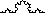
\includegraphics[width=0.3\textwidth]{../images/koch-line-03.pdf}
  \hfill
  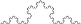
\includegraphics[width=0.3\textwidth]{../images/koch-line-04.pdf}
  \hfill
  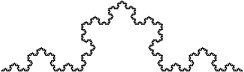
\includegraphics[width=0.3\textwidth]{../images/koch-line-05.pdf}
  \hfill
  \caption{Segunda iteração da construção da linha de Koch.}
\end{figure}


Continuando com o mesmo procedimento em cada passo, no limite obtém-se
a figura designada por linha de Koch. Assumimos, sem demonstração, que
existe efectivamente o limite desta sucessão.

A linha de Koch tem, entre outras, as seguintes propriedades
interessantes:


\begin{itemize}

\item É uma linha contínua.

\item Não tem derivada em nenhum ponto. Tomamos aqui a linha como uma
  aplicação de $\mathbb{R} \to \mathbb{R}^2$.

\item Tem comprimento infinito.

\end{itemize}


É simples verificar que o comprimento da linha de Koch é infinito. De
facto, se chamarmos ao comprimento da figura do passo n tem-se que

\[ L_n = \frac{4}{3}L_{n-1} \]

Como $L_0=1$  então

\[ L_n = \left(\frac{4}{3}\right)^n, \]
que é uma sucessão que cresce sem ter majorante. Ou seja, o
comprimento da figura limite é infinito.





\section{Ilha de Koch}

A figura conhecida como ilha de Koch é obtida através de um
procedimento semelhante ao usado para criar a linha de Koch, mas em
vez de começar com um único segmento começa-se com um triângulo
equilátero. As imagens em baixo representam as seis primeiras
iterações do procedimento.


O perímetro da ilha de Koch é infinito. Tal acontece porque esta
figura é constituida pela união de três versões idênticas,
apropriadamente rodadas e deslocadas, da linha de Koch. No entanto a
área da ilha de Koch é claramento limitada. Podemos mesmo calcular a
área como o limite da sucessão das áreas das figuras intermédias.

A área da ilha de Koch pode ser obtida como o limite das áreas das
figuras intermédias. Vamos então calcular a área $A_n$ da figura
do passo n. A área da figura do passo n é dada pela soma da área da
figura do passo n-1 com as áreas dos pequenos triângulos que são
adicionados à figura do passo n-1 para obter a figura do passo n.

Precisamos de saber quantos pequenos triângulos são acrescentados no
passo n-1 para obter a figura do passo n. Precisamos também de saber o
comprimento do lado desses pequenos triângulos, para calcular a
respectiva área.

O número de pequenos triângulos que são acrecentados no passo $n-1$
corresponde ao número de troços no passo $n-1$. Chamemos $c_n$ ao
número de troços no passo $n$. Tem-se então:

\[c_0=3, \quad c_n=4c_{n-1} \qquad \Rightarrow \qquad c_n = 3\times 4^n \]

O comprimento do lado dos pequenos triângulos que são acrescentados no
passo n-1 corresponde ao número de troços que existem no passo
n. Chamemos-lhe $l_n$. Tem-se que:

\[
 l_0=1, 
\quad l_n=\frac{1}{3}l_{n-1}
\qquad \Rightarrow
\qquad l_n = \left(\frac{1}{3}\right)^n
\]

Chamemos $a_n$ à área de cada um dos pequenos triângulos acrescentados
no passo $n-1$. Sendo a área a de um triângulo equilátero de lado $l$ dada
por $a=\frac{\sqrt{3}}{4}l^2$ teremos

\[
a_n = \frac{\sqrt{3}}{4} l_n^2 = \frac{\sqrt{3}}{4} \left(\frac{1}{9}\right)^n
\]

Com o que já foi dito temos

$latex \displaystyle A_n = A_{n-1} + c_{n-1}a_n $

$latex \displaystyle A_n = A_0 + \sum_{k=1}^n c_{k-1}a_k $

$latex \displaystyle A_n = \frac{\sqrt{3}}{4} \left( 1 + \frac{3}{4} \sum_{k=1}^n \left(\frac{4}{9}\right)^n \right)$

No limite temos a soma dos termos de uma progressão geométrica de razão 4/9. Sendo $latex \sum_{k=0}^\infty = \frac{1}{1-r}$ ou $latex \sum_{k=1}^\infty = \frac{r}{1-r}$ teremos finalmente a área da ilha de Koch como

$latex \displaystyle A = \lim A_n = \frac{2\sqrt{3}}{5} $

Cólofon

As imagens PNG usadas neste artigo com os diferentes passos das iterações da linha de Koch e ilha de Koch foram geradas com Inkscape a partir de ficheiros SVG.

Os ficheiros SVG com as figuras foram gerados a partir de um programa para geração de iterações de Sistemas-L escrito na linguagem de scripting Tea.

  




  






\end{document}

